\documentclass{beamer}
\usetheme{Madrid}
\usecolortheme{default}
\usepackage{ctex}
\usepackage{ulem}
\usepackage{amsmath}
\usepackage{hyperref}
\usepackage{graphicx}
\usepackage{media9}
\title{行星吸积大气}
\author{董桁宇}
\date{\today}
\begin{document}
\section{Title}
\frame{\titlepage}
\begin{frame}
\frametitle{Preface}
The author of this slides is:\\
董桁宇(Hengyu Dong)\\
This sides is based on the paper called\\
\begin{center} 
ATMOSPHERES OF PROTOPLANETARY CORES: CRITICAL MASS FOR NUCLEATED INSTABILITY\\ 
Roman R. Rafikov\\
{\tiny Institute for Advanced Study, Einstein Drive, Princeton, NJ 08540; rrr@cita.utoronto.ca}
\end{center}
from\\
\begin{center}
The Astrophysical Journal, 648:666Y682, 2006 September 1\\
{\tiny \textcircled{c} 2006. The American Astronomical Society. All rights reserved. Printed in U.S.A}
\end{center}
You can find this slides on \href{https://github.com/little-potato-loria/the-pre-of-astrophysics}{董桁宇(Hengyu Dong)'s github}\\
{\tiny This work is licensed under a \href{https://creativecommons.org/licenses/by-nc/4.0/}{Creative Commons Attribution-NonCommercial 4.0 International License}.}
\end{frame}

\begin{frame}
\frametitle{Outline}
\tableofcontents
\end{frame}

\section{Setting up}
\begin{frame}
\frametitle{Settings}
Settings about the nebula:\\
MMSN (Minimum Mass Solar Nebula):\\
$\Sigma_p(a)$ is the particulate surface densities\\
$\Sigma_g(a)$ is the gas surface densities\\
$T_0(a)$ is the gas temperature \\
$a_n \equiv a/(n \, \text{AU})$, while 'a' is the distance to the sun
\begin{equation}
\Sigma_g(a) \approx 100 \Sigma_p(a) \approx 3000 \, \text{g cm}^{-2} \, a_1^{-3/2}
\end{equation}
\begin{equation}
T_0(a) \approx 300 \, \text{K} \, a_1^{-1/2}
\end{equation}
\end{frame}

\begin{frame}
\frametitle{Settings}
The nebula is isothermal in the vertical direction\\ 
$\rho(z,a) = \rho_0(a) \exp(-z^2/2h^2)$ is the density structure\\ 
$c_0 \equiv (kT_0/\mu)^{1/2}$ is the isothermal sound speed\\ 
$k$ is the Boltzmann constant and $\mu$ is the mean molecular weight\\ 
$h \equiv c_0/\Omega$ is the vertical scale height\\ 
$\Omega \equiv (GM_\odot/a^3)^{1/2}$ is the orbital angular frequency\\ 
$\rho_0 \equiv (2\pi)^{-1/2}\Sigma_g/h$ is the midplane density\\
In terms of numbers:
\begin{equation}
c_0(a) \approx 10^5 \, \text{cm s}^{-1} \, a_1^{-1/4}
\end{equation}
\begin{equation}
h(a)/a \approx 3.4 \times 10^{-2} \, a_1^{1/4}
\end{equation}
\begin{equation}
\rho_0(a) \approx 2.4 \times 10^{-9} \, \text{g cm}^{-3} \, a_1^{-11/4}
\end{equation}
\end{frame}

\begin{frame}
\frametitle{Basic equations}
Assume that:\\
the atmosphere is not rapidly rotating\\
the gas distribution as spherically symmetric\\
$M_p \gtrsim M_{atm}$\\
we can get:
\begin{equation}
\frac{\partial P}{\partial r} =  -G\frac{M_p}{r^2}\rho
\end{equation}
$M_p$means the mass of the core embedded in the nebular gas.
$M_{atm}$means the mass of the atmosphere.
\end{frame}

\begin{frame}
\frametitle{Basic equations}
Assume that:\\
{\small the planetesimal velocity far from the core is small compared to the core’s escape speed\\
planetesimals penetrate to the core surface without much resistance from the envelope and release there all their kinetic energy\\
the dynamical and thermal timescales of the atmosphere are shorter than the core accretion timescale $\frac{Mp}{\dot{M}}$\\}
we can get:
\begin{equation}
L = -G\frac{M_p \dot{M}}{R_p}
\end{equation}
$R_p$means the radio of the core embedded in the nebular gas.\\
{\small However, even in the most unfavorable case of small planetesimals that are quasi-statically lowered from the top of the atmosphere to its bottom, 
the luminosity is $1 - \frac{R_p}{r}L$\\
i.e., the luminosity varies only very near the core’s surface. At $r \gtrsim R_p$, in the bulk of the atmosphere, we can safely assume L to be a constant given by the equation.}
\end{frame}

\begin{frame}
\frametitle{Basic equations}
Assume that:\\
the envelope is chemically homogeneous\\
the envelope is nonrotating\\
we can get:
\begin{equation}
\frac{\partial ln T}{\partial ln P} \equiv \nabla < \nabla_{ad} \equiv \frac{\gamma-1}{\gamma}
\end{equation}
$\nabla$means the temperature gradient.\\
$\nabla_{ad}$means the temperature gradient under isentropic conditions.\\
$\gamma$means the adiabatic index of the gas.\\
Imagining a small part of the gas was slightly disturbed.\\
This equation can be used to determine weather the accretion luminosity is transported by radiative diffusion or convection.
\end{frame}

\begin{frame}
\frametitle{Basic equations}
Assume that:\\
optically thick\\
the dynamical and thermal timescales of the atmosphere are shorter than the core accretion timescale $\frac{Mp}{\dot{M}}$\\
we can get:
\begin{equation}
\frac{16\sigma T^3}{3\kappa \rho}\frac{\partial T}{\partial r}=-\frac{L}{4\pi r^2}
\end{equation}
$\sigma$ is the Stefan-Boltzmann constant.\\
$\kappa$ is the opacity.\\
we assume that:
\begin{equation}
\kappa=\kappa_{0} \frac{P}{P_0}^\alpha \frac{T}{T_0}^\beta
\end{equation}
$\kappa_0,P_0,T_0$ are the opacity, pressure, and temperature in the nebular gas far from the core.\\
And we assume that $\kappa_0$ is independent of a.
\end{frame}

\begin{frame}
\frametitle{Basic equations}
Assume that:\\
the envelope is chemically homogeneous\\
the envelope is ideal gas\\
we can get:
\begin{equation}
\tag{0}
P = C_{onst} \rho T
\end{equation}
And if the equation(8)$(\nabla < \nabla_{ad})$is violated\\
$\nabla \approx \nabla_{ad}$
we can get:
\begin{equation}
P=C_{onst} \rho ^ \gamma
\end{equation}
\end{frame}

\section{Scales}
\begin{frame}
\frametitle{Length Scales}
The mean free path of photons in the nebular gas:
\begin{equation}
\lambda = {(\kappa_0 \rho_0)}^{-1} \equiv 1.7 \times 10^9 \, \text{cm} \, a_1^{11/4} \kappa_{0.1}^{-1}
\end{equation}
The Hill radius:
\begin{equation}
R_H \equiv a \left( \frac{M_p}{M_\odot} \right)^{1/3} \approx 2 \times 10^{11} \, \text{cm} \, a_1 \left( \frac{M_p}{M_\oplus} \right)^{1/3}
\end{equation}
This equation can be used to determine whether the gas is controlled by the gravity of the core or the star.
The Bondi radius:
\begin{equation}
R_B \equiv \frac{G M_p}{c_0^2} \approx 4 \times 10^{10} \, \text{cm} \, a_1^{1/2} \frac{M_p}{M_\oplus}
\end{equation}
is defined as the distance from the protoplanet at which the thermal energy of the nebular gas is of the order of its gravitational energy in the potential well of the core. ($P \approx P_0$ when $r \gtrsim R_B$)
\end{frame}

\begin{frame}
\frametitle{Length Scales}
The radius of the core:
\begin{equation}
R_p \equiv \left( \frac{3}{4 \pi} \frac{M_p}{\rho_p} \right)^{1/3} \approx 10^9 \, \text{cm} \left( \frac{M_p}{M_\oplus} \right)^{1/3} \rho_1^{-1/3}
\end{equation}
\begin{equation}
p \equiv \frac{R_p}{R_H} = \left( \frac{3 M_\odot}{4 \pi \rho_p a^3} \right)^{1/3} \approx 5.2 \times 10^{-3} a_1^{-1} \rho_1^{-1/3} 
\end{equation}
where $\rho_1 \equiv \rho_p (1 \, \text{g} \, \text{cm}^{-3})$ and $R_p \gg R_H$\\
The luminosity radius:
\begin{equation}
R_L \equiv \left( \frac{L}{16 \pi \sigma T_0^4} \right)^{1/2}
\end{equation}
The luminosity radius is 1/2 of the radius of the sphere that can radiate the accretion luminosity L at an effective temperature T
\end{frame}

\begin{frame}
\begin{columns}[t] 
\begin{column}{0.6\textwidth} 
\vspace{-0.5cm}
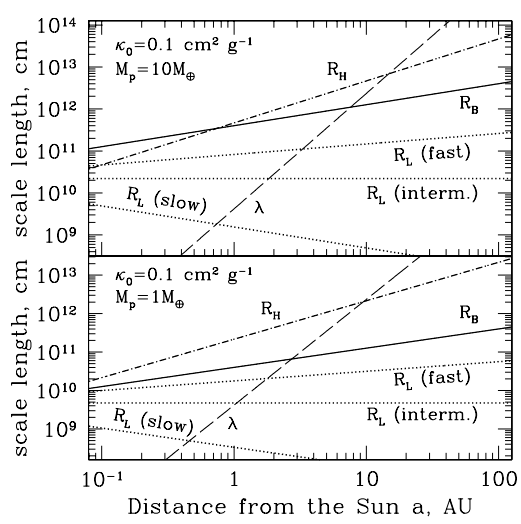
\includegraphics[width=\textwidth]{length_scale.png}
{\small Dotted lines correspond to the luminosity radius $R_L$ evaluated for three different planetesimal accretion regimes, fast, intermediate, and slow.}
\end{column} 
\begin{column}{0.4\textwidth}
We define the "sphere of influence"as the region of space in which planetary gravity dominates over both the tidal field of the Sun and the unperturbed nebular pressure $P_0$.\\
\hspace*{\fill} \\
{\Large It is min($R_H,R_B$)}\\
\hspace*{\fill} \\
The gas dynamics inside it is determined only by the gravity of the core and pressure gradients in the surrounding gas.
\end{column} 
\end{columns}
\end{frame}

\begin{frame}
\frametitle{Mass Scales}
Atmosphere exists $\iff R_B \gtrsim R_p \iff M_p \gtrsim M_a$:
\begin{equation}
M_a \equiv \frac{c_0^3}{G}\left( \frac{3}{4 \pi G \rho_p} \right)^{1/2} \approx 4.5 \times 10^{-3} M_{\oplus} a_1^{-3/4} \rho_1^{-1/2}
\end{equation}
The nebula can be considered homogeneous on the scale of $R_B$ \\
$\iff R_B \ll h \iff M_p \lesssim M_{tr}$
\begin{equation}
M_{tr} \equiv \frac{c_0^3}{G \Omega} \approx 12 M_{\oplus} a_1^{3/4}
\end{equation}
We can see that: $R_B \lesssim R_H$ and $R_H \lesssim h$, if $R_B \ll h$ \\
$R_B \gtrsim R_H$ and $R_H \gtrsim h$, if $R_B \gg h$ \\
Now we only talk about the situation that:
\begin{equation}
M_a \lesssim M_p \lesssim M_{tr}
\end{equation}
\begin{equation}
R_p \lesssim R_B \lesssim R_H \lesssim h
\end{equation}
\end{frame}

\begin{frame}
\begin{columns}[t] 
\begin{column}{0.6\textwidth} 
\vspace{-0.5cm}
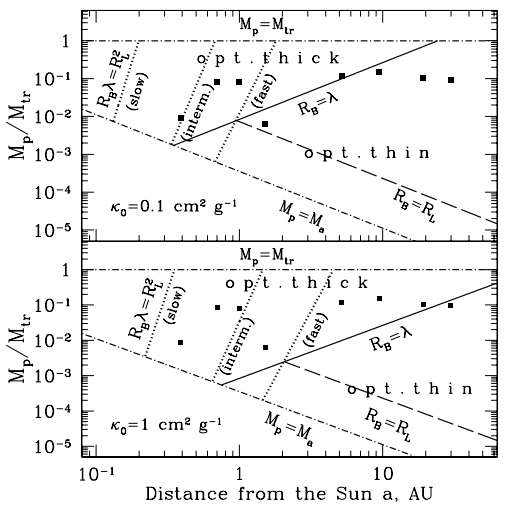
\includegraphics[width=\textwidth]{mass_scale.png}
{\small Dotted lines correspond to the luminosity radius $R_L$ evaluated for three different planetesimal accretion regimes, fast, intermediate, and slow.}
\end{column} 
\begin{column}{0.4\textwidth}
Since according to equations (18) and (19) $M_a = p^{3/2} M_{tr}$, there is a broad mass range in which equation (20) can be valid, spanning 4-5 orders of magnitude in mass depending on a (e.g., from ~0.1 lunar mass to ~$M_J$ at 10 AU ). 
\end{column} 
\end{columns}
\end{frame}

\section{Low-Luminosity}
\begin{frame}
\frametitle{Low-Luminosity Optically Thick}
we define:
\begin{equation}
T(R_{out})=T_0,P(R_{out})=P_0,\rho(R_{out})=\rho_0,
\end{equation}
The core is "low-luminosity" if any of the following equations holds true.\\
For the Optically Thick case:
\begin{equation}
\lambda \ll R_B , {R_L}^2 \ll \lambda R_B
\end{equation}
For the Optically Thin case:
\begin{equation}
R_L \ll R_B \ll \lambda
\end{equation}
using equations (6) (8) (9),we get:
\begin{equation}
\nabla(T) = \frac{3}{64\pi} \frac{L\kappa_0 \rho_0 {c_0}^2}{GM_p\sigma {T_0}^4} {(\frac{T}{T_0})}^{\beta-4} {(\frac{P}{P_0})}^{1+\alpha}=\nabla_{\infty}{(\frac{T}{T_0})}^{\beta-4} {(\frac{P}{P_0})}^{1+\alpha}
\end{equation}
\begin{equation}
\nabla_{\infty}=\frac{3}{4} \frac{{R_L}^2}{R_B \lambda}
\end{equation}
As we can see $\nabla(T)=\nabla_{\infty}$in the outer atmosphere.
\end{frame}

\begin{frame}
\frametitle{Low-Luminosity Optically Thick}
Using equation (6)(9)(10),we can get:
\begin{equation}
{(\frac{P}{P_0})}^{1+\alpha}-1=\frac{\nabla_0}{\nabla_\infty}[{(\frac{T}{T_0})}^{4-\beta}-1]
\end{equation}
\begin{equation}
\nabla_0 \equiv \frac{1+\alpha}{4-\beta}
\end{equation}
Because of equation (23),$\frac{\nabla_0}{\nabla_\infty}$is really big, which means that a large change of P results in only a small perturbation of T.\\
Later we will talk about the asymptotic behavior of the atmospheric properties in two regions: \\
in the "outer atmosphere", where$ T-T_0\lesssim T_0(T \approx T_0)$, \\
and in the "deep atmosphere", where one expects $T \gg T_0$.
\end{frame}

\begin{frame}
\frametitle{Low-Luminosity Optically Thick}
In the "outer atmosphere", $ T-T_0\lesssim T_0$, substituting equation (27) into either equation (6) or equation (9)we can get:
\begin{equation}
\frac{P}{P_0}\approx\frac{\rho}{\rho_0}\approx e^{(\frac{R_B}{r}-\frac{R_B}{R_{out}})}\approx e^{\frac{R_B}{r}}
\end{equation}
\begin{equation}
\frac{T-T_0}{T_0}\approx \frac{\nabla_{\infty}}{1+\alpha}(e^{(1+\alpha)(\frac{R_B}{r}-\frac{R_B}{R_{out}})}-1)\approx \frac{\nabla_{\infty}}{1+\alpha}(e^{(1+\alpha)\frac{R_B}{r}}-1)
\end{equation}
\end{frame}

\begin{frame}
\frametitle{Low-Luminosity Optically Thick}
When $T-T_0 \sim T_0$ according to equation (30),"outer atmosphere" turn to "deep atmosphere",the radio is :
\begin{equation}
R_a\equiv R_B\frac{1+\alpha}{ln(R_B \lambda/{R_L}^2)}\approx R_B \frac{1+\alpha}{ln({\nabla_{\infty}}^{-1})}
\end{equation}
so the pressure and density is
\begin{equation}
\frac{P_a}{P_0}\approx\frac{\rho_a}{\rho_0}\approx {\nabla_{\infty}}^{-1/(1+\alpha)}\gg 1
\end{equation}
\end{frame}

\begin{frame}
\frametitle{Low-Luminosity Optically Thick}
In the "deep atmosphere",$ T \gg T_0$, with boundary condition that$T \approx \xi T_0 at r =R_a$ substituting equation (27) into either equation (6) or equation (9)we can get:
\begin{equation}
\frac{T}{T_0}\approx \xi +\nabla_0 (\frac{R_B}{r}-\frac{R_B}{R_a})
\end{equation}
\begin{equation}
\frac{P}{P_0}\approx (\frac{\nabla_0}{\nabla_{\infty}})^{1/(1+\alpha)}[\xi +\nabla_0 (\frac{R_B}{r}-\frac{R_B}{R_a})]^{1/\nabla_0}
\end{equation}
\end{frame}

\begin{frame}
\frametitle{Low-Luminosity Optically Thick}
\begin{columns}[t] 
\begin{column}{0.5\textwidth} 
It can also be calculated numerically, the result is:
\vspace{-0.1cm}
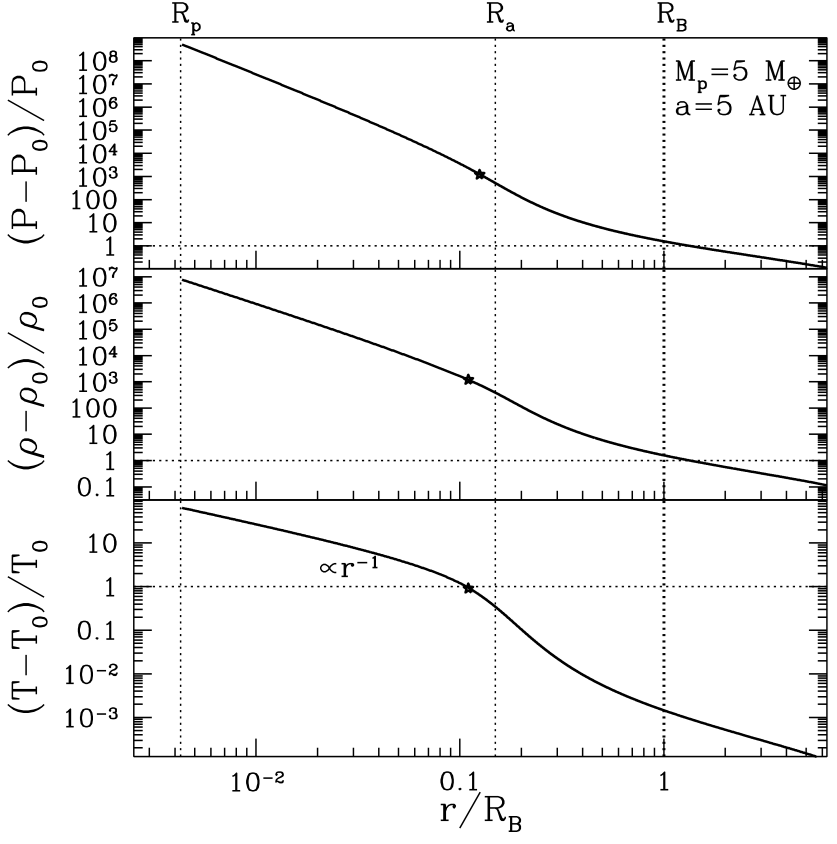
\includegraphics[width=\textwidth]{Low-Luminosity Optically Thick.png}
\end{column} 
\begin{column}{0.5\textwidth}
$M_p=5 M_{\oplus},a=5AU,P_0 =1.3 \times 10^{-7} \text{bar}, \rho_0 =3 \times 10^{-11} \text{g cm}^{-3},T_0= 130 \text{K}, \alpha=0, \beta=1, \gamma = \frac{7}{5}, \kappa_0=0.1 \text{cm}^2 \text{g}^{-1}$, planetesimal accretion is in the intermediate regime.
\begin{equation}
\tag{A1}
\dot{M}=\Omega \Sigma_p R_P R_H \theta
\end{equation}
\begin{equation}
\tag{A2}
\scriptscriptstyle \tau_{acc}\equiv \frac{M_p}{\dot{M}}=\frac{M_p}{\Omega \Sigma_p R_P R_H}\theta^{-1} \approx (\frac{M_p}{M_{\oplus}})^{1/3} \left\{ \begin{array}{ll}\scriptscriptstyle 3 \times 10^{10} \, \text{yr} \, a_{10}^3, & \text{slow}, \\ \scriptscriptstyle 1.4 \times 10^7 \, \text{yr} \, a_{10}^2, & \text{intermediate}, \\ \scriptscriptstyle 3 \times 10^5 \, \text{yr} \, a_{10}^{3/2}, & \text{fast}. \end{array} \right\}
\end{equation}
\end{column} 
\end{columns}
\end{frame}

\begin{frame}
\frametitle{Low-Luminosity Optically Thick}
I have written a c program and a shell to reproduce the image.The program can be found on \href{https://github.com/little-potato-loria/plot2.git}{董桁宇(Hengyu Dong)'s github}
 And the results fit well.
\end{frame}

\begin{frame}
\frametitle{Low-Luminosity Optically Thin}
When $\lambda \gtrsim R_B$ the boundary will be optically thin.Deep in the atmosphere (below the photosphere) the gas becomes optically thick because of the increasing density ,while the nebula is also optically thick when$r\gg \lambda$ because it is "thick",so it is:
\begin{table}
\centering
\begin{tabular}{|c|c|c|}
\hline
0 to $R_{ph}$ & $R_{ph} to \lambda$ & $\lambda to \infty$\\
\hline
thick & thin & think \\
\hline
\end{tabular}
\end{table}
And equation (9) can not be used in the optically thin area.Insteadly, it should be$ T^4\approx {T_0}^4 +L/(16 \pi \sigma r^2)$ then we interpolating between the outer optically thick and intermediate optically thin regions,we get:
\begin{equation}
T^4 (r) \approx {T_0}^4 (r)+\frac{L}{16 \pi \sigma r^2}+\frac{3L}{16 \pi \sigma}\int_{r}^{\infty}\frac{\kappa \rho(r')dr'}{{r'}^2}
\end{equation}
\end{frame}

\begin{frame}
\frametitle{Low-Luminosity Optically Thin}
Because of $R_L \ll R_B \ll \lambda$,we can get that when $r \gtrsim R_B$
\begin{equation}
T (r) \approx T_0{(1+\frac{{R_L}^2}{r^2}+3\frac{{R_L}^2}{\lambda r})}^{1/4}
\end{equation}
When $r =R_B$ , from equation (36) ,we can get $T(R_B)-T_0 \sim T_0(R_L /R_B)^2$\\
Because $T\approx T_0$.P and $\rho$ follow equation(29).
\end{frame}

\begin{frame}
\frametitle{Low-Luminosity Optically Thin}
Define $R_{ph}$ as the radius that $\lambda = \partial r/\partial ln P$,while$\partial r/\partial ln P=r^2/R_B$ according to equation(29), So $R_{ph}$ actually means the radius that the atmosphere change from thin to thick.
\begin{equation}
R_{ph} \approx R_B \frac{1+\alpha}{ln(\lambda /R_B)}
\end{equation}
So we can get:$T_{ph} \equiv T(R_{ph}),P_{ph} \equiv P(R_{ph})$
\begin{equation}
\frac{T_{ph}-T_0}{T_0} \approx \frac{{R_L}^2}{4 {R_{ph}}^2} \approx  [\frac{ln(\lambda/R_B)}{2(1+\alpha)}\frac{R_L}{R_B}]^2 \ll 1
\end{equation}
\begin{equation}
P_{ph}/P_0 \approx (\lambda/R_B)^{1/(1+\alpha)} \gg 1
\end{equation}
\end{frame}

\begin{frame}
\frametitle{Low-Luminosity Optically Thin}
When$r< R_{ph}$,the atmosphere is optically thick,from equation (27) we can get:
\begin{equation}
(\frac{P}{P_0})^{1+\alpha}-(\frac{P_{ph}}{P_0})^{1+\alpha}=\frac{\nabla_0}{\nabla_{\infty}}
[(\frac{T}{T_0})^{4-\beta}-(\frac{T_{ph}}{T_0})^{4-\beta}]
\end{equation}
\begin{equation}
\frac{T-T_{ph}}{T_0}=\frac{\nabla_{\infty}}{(1+\alpha)}
[e^{(1+\alpha)\frac{R_B}{r}}-(\frac{R_{ph}}{P_0})^{1+\alpha}]
\end{equation}
\end{frame}

\begin{frame}
\frametitle{Low-Luminosity Optically Thin}
\begin{columns}[t] 
\begin{column}{0.5\textwidth} 
It can also be calculated numerically, the result is:
\vspace{-0.1cm}
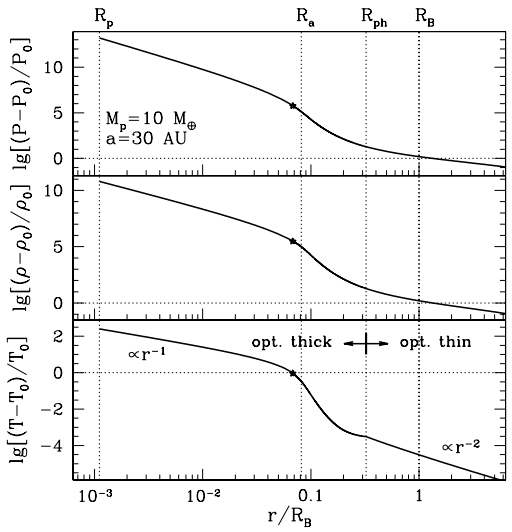
\includegraphics[width=\textwidth]{Low-Luminosity Optically Thin.png}
\end{column} 
\begin{column}{0.5\textwidth}
$M_p=10 M_{\oplus},a=30AU,P_0 =4 \times 10^{-10} \text{bar}, \rho_0 =2 \times 10^{-13} \text{g cm}^{-3},T_0= 55 \text{K}, \alpha=0, \beta=1, \gamma = \frac{7}{5}, \kappa_0=0.1 \text{cm}^2 \text{g}^{-1}$, planetesimal accretion is in the intermediate regime.
\end{column} 
\end{columns}
\end{frame}

\begin{frame}
\frametitle{Low-Luminosity Convection in the Deep Atmosphere}
For the "optically thick" case, from equation (25) and (27)we can get:
\begin{equation}
\nabla(T)=\nabla_0[1-(\frac{T_0}{T})^{4-\beta}(1-\frac{\nabla_{\infty}}{\nabla_0})]
\end{equation}
We have said that $\frac{\nabla_{\infty}}{\nabla_0}$is really small,so:
\begin{equation}
\nabla(T) \approx \nabla_0[1-(\frac{T_0}{T})^{4-\beta}]
\end{equation}
And we can see that :\\
when $T \approx T_0 , \nabla(T) \approx 0 \ll \nabla_{ad}$\\
when $T \gg T_0 , \nabla(T) \approx \nabla_0 $
\end{frame}

\begin{frame}
\frametitle{Low-Luminosity Convection in the Deep Atmosphere}
For the "optically thick" and $r > R_{ph}$ case, using the definition of $\nabla = \frac{\partial ln T}{\partial ln P}$ the equation (29) and (36) with the approximate relationship $ ln(1+d) \approx d$,we can get:
\begin{equation}
\nabla \approx \frac{1}{4}(2\frac{{R_L}^2}{R_B r}+3\frac{{R_L}^2}{R_B \lambda}) \ll 1
\end{equation}
And for the "optically thick" and $r \lesssim R_{ph}$ case,same as equation (42),we can get:
\begin{equation}
\nabla(T)=\nabla_0[1-(\frac{T_{ph}}{T})^{4-\beta}(1-\frac{\nabla_{\infty}}{\nabla_0}(\frac{P_{ph}}{P_0})^{1+\alpha}(\frac{T_0}{T_{ph}})^{4-\beta})]
\end{equation}
With the $ T_{ph} R_{ph}$ we have already calculated, equation (45) equal  to equation (43). Thus we prove that the upper atmosphere must be radiative .
\end{frame}

\begin{frame}
\frametitle{Low-Luminosity Convection in the Deep Atmosphere}
As we have proved the temperature gradient in the deep atmosphere is $\nabla_0$ ,the \textbf{whole} atmosphere is convectively stable if 
\begin{equation}
\nabla_0 < \nabla_{ad}
\end{equation}
With the equation (43) we can define $T_{conv} $ as the temperature that $\nabla $ = $\nabla_{ad}$, so we can get:
\begin{equation}
T_{conv} \approx T_0{(1-\frac{\nabla_{ad}}{\nabla_0})}^{-1/(4-\beta)}
\end{equation}
We have said that $\frac{\nabla_{\infty}}{\nabla_0}$is really small,so $T_{conv} \approx T_0 $so r $\approx R_a$
\end{frame}

\begin{frame}
\frametitle{Low-Luminosity Convection in the Deep Atmosphere}
Taking the equation (47) into equation (40),we can get $P_{conv}$
\begin{equation}
\begin{split}
P_{conv} &  \equiv P_0[{(\frac{P_{ph}}{P_0})}^{1+\alpha}+\frac{\nabla_0}{\nabla_{\infty}}(\frac{1}{1-\nabla_{ad}/\nabla_0}-{(\frac{T_{ph}}{T_0})}^{4-\beta})]^{1/(1+\alpha)}\\
& \approx P_0 {[\frac{\nabla_{ad}\nabla_0}{\nabla_{\infty}(\nabla_0-\nabla_{ad})}]}^{1/(1+\alpha)}
\end{split}
\end{equation}
Because equation (39) and$ T_{ph} \approx T_0 $ and ${\nabla_{\infty}}^{-1} \ll \lambda/R_B$\\
And from equation (32),we can get$P_{conv} \sim P_a \gg P_0$\\
And$\rho_{conv}$ can be calculated by equation (6)and (11)with boundary condition $ \rho_{conv} at R_a$:
\begin{equation}
\begin{split}
\rho(r)& =\rho_{conv}{[1+\nabla_{ad}\frac{GM_p}{K{\rho_{conv}}^{\gamma-1}}(\frac{1}{r}-\frac{1}{R_a})]}^{1/(\gamma-1)}\\
&=\rho_{conv}{[1+\nabla_{ad}{(1-\frac{\nabla_{ad}}{\nabla_0})}^{1/(4-\beta)}(\frac{R_B}{r}-\frac{R_B}{R_a})]}^{1/(\gamma-1)}
\end{split}
\end{equation}
\end{frame}

\begin{frame}
\frametitle{Low-Luminosity Convection in the Deep Atmosphere}
When $r \lesssim R_a(1-R_a/R_B),\rho \gg \rho_{conv}$ we can get:
\begin{equation}
{(\frac{\rho}{\rho_{conv}})}^{\gamma-1} \approx \frac{T}{T_{conv}} \approx \nabla_{ad}\frac{T_0}{T_{conv}}(\frac{R_B}{r}-\frac{R_B}{R_a})
\end{equation}
Which is similar to equation (33) $\xi + \nabla_0 (\frac{R_B}{r}-\frac{R_B}{R_a})$
\end{frame}

\section{High-Luminosity}
\begin{frame}
\frametitle{High-Luminosity Optically Thin}
The core is "high-luminosity" if any of the following equations holds true.\\
For the Optically Thick case:
\begin{equation}
\lambda \ll R_B , {R_L}^2 \gtrsim \lambda R_B
\end{equation}
For the Optically Thin case 
\begin{equation}
\tag{54}
R_L \gg R_B , \lambda \gg R_B 
\end{equation}
When it is Optically Thin,according to equation(36),T is strongly perturbed even $r>R_B$.
\end{frame}

\begin{frame}
\frametitle{High-Luminosity Optically Thick}
Now we will talk about the Optically Thick case, from equation (25),$\nabla_{\infty} \gtrsim \nabla_{ad}$,so the outer convective zone exists.\\
Same as what we did in equation (49) but $R_a$and$\rho_{conv}$turn to $R_{out}$and$\rho_0$ , besides, $T_0=T_{conv}$
\begin{equation}
\rho(r)=\rho_0{[1+\nabla_{ad}(\frac{R_B}{r}-\frac{R_B}{R_{out}})]}^{1/(\gamma-1)}
\end{equation}
which shows that $\rho$, P, and T deviate by a factor of $\sim$ 1 from $\rho_0, P_0, T_0 $at $ r \sim R_B$
\end{frame}

\begin{frame}
\frametitle{High-Luminosity Optically Thick}
However, in the deep atmosphere it depends on $\nabla_0$and$\nabla_{\infty}$.\\
When $\nabla_0 > \nabla_{\infty}$,the atmosphere is wholly convective;\\
when $\nabla_0 < \nabla_{\infty}$,the outer atmosphere is convective but the inner atmosphere is radiative.\\
We can calculate $\nabla(T)$ same as equation (45) with different boundary condition given by equation(52),then the radius when $\nabla(T)=\nabla_{ad}$ is $R_{rad}$:
\begin{equation}
R_{rad} \approx R_B \frac{\nabla_{ad}}{\Theta},\Theta \equiv {(\frac{\nabla_{\infty}}{\nabla_{ad}})}^{\nabla_{ad}/[(4-\beta)(\nabla_{ad}-\nabla_0)]}
\end{equation}
We can see that$R_{rad} \ll R_B$($\nabla_{\infty} \gtrsim \nabla_{ad}$).\\
$R_{rad}>R_B$ is also required for the establishment of the inner radiation zone.\\
When $\rho_{rad} \gg \rho_0 ,T_{rad}/T_0={(\rho_{rad}/\rho_0)}^{\gamma-1} \approx \Theta $ 
\end{frame}

\begin{frame}
\frametitle{High-Luminosity Optically Thick}
\begin{columns}[t] 
\begin{column}{0.5\textwidth} 
\vspace{-0.1cm}
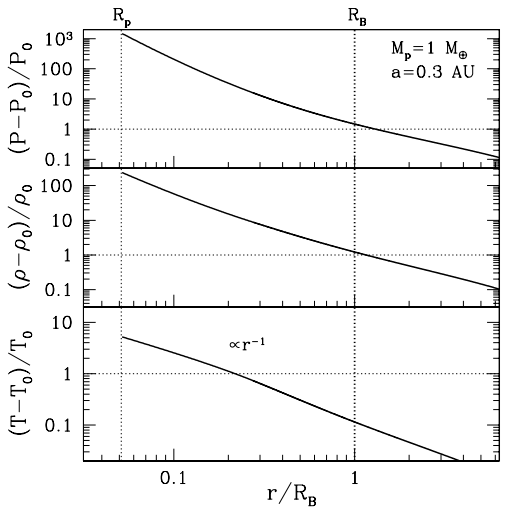
\includegraphics[width=\textwidth]{High-Luminosity Optically Thick.png}
\end{column} 
\begin{column}{0.5\textwidth}
$M_p=1 M_{\oplus},a=0.3AU,P_0 = 10^{-3} \text{bar}, \rho_0 =7 \times 10^{-8} \text{g cm}^{-3},T_0= 550 \text{K}, \alpha=0, \beta=1, \gamma = \frac{7}{5}, \kappa_0=0.1 \text{cm}^2 \text{g}^{-1}$, planetesimal accretion is in the intermediate regime.\\
This case is High-Luminosity Optically Think Wholly Convective
\end{column} 
\end{columns}
\end{frame}

\section{Mass of Atmosphere}
\begin{frame}
\frametitle{Mass of Low-Luminosity Atmosphere}
The mass of atmosphere $M_{atm}$ is define as:
\begin{equation}
\tag{55}
M_{atm} \equiv 4\pi \int_{R_p}^{R_B} \rho(r) r^2 dr
\end{equation}
So for the optically thick case, $\rho$ drops exponentially outside $R_a$ ,so we can replace the $R_B$ of equation (55) into$R_a$,so that $M_{atm}$ can be calculated by equation (33)(34)(radiative)or(47)(48)(50)(convective):
\begin{equation}
\tag{56}
M_{atm}  \approx 4 \pi \Psi_1 \rho_0 {R_B}^3 {(\frac{R_B \lambda}{R_L^2})}^{1/(1+\alpha)}
\end{equation}
\begin{equation}
\tag{B1}
\Psi_1 \approx C {(\frac{R_a}{R_B})}^{3-\varsigma} \int_{0}^{1} z^2{(\frac{1}{z}-1)}^\zeta dz
\end{equation}
We have set $R_p/R_B$ to 0.\\
\end{frame}

\begin{frame}
\frametitle{Mass of Low-Luminosity Atmosphere}
For the radiative case :
\begin{equation}
\tag{B2}
C = \left( \frac{4 \nabla_0}{3} \right)^{1/(1+\alpha)} \nabla_0^{(1 - \nabla_0)/\nabla_0}, \quad \zeta = \frac{1}{\nabla_0} - 1,
\end{equation}
For the convective case :
\begin{equation}
\tag{B3}
C = \left( 1 - \frac{\nabla_{\text{ad}}}{\nabla_0} \right)^{1/\nabla_{\text{ad}}(4 - \beta)} \left( \frac{4 \nabla_0 \nabla_{\text{ad}}}{3 \nabla_0 - \nabla_{\text{ad}}} \right)^{1/(1+\alpha)} \nabla_{\text{ad}}^{1/(\gamma - 1)}, \quad \zeta = \frac{1}{\gamma - 1}.
\end{equation}
$\zeta$ is the power-law index of 1/r,and we will plus $r^2$ and then integrate.\\
When $\zeta < 3$,the main part of $M_{atm}$ comes from $r \sim R_a$ and it is weakly depends on smaller r.\\
When $\zeta = 3 , \alpha =0$,each decade in radius have same mass, so we will change equation (B1) into $\Psi \sim ln(R_a/R_p)$.\\
When $\zeta > 3$,the main part of$M_{atm}$ comes from the innermost part of the atmosphere near $R_p$ and $M_{atm} \propto {(R_a/R_p)}^{\zeta-3}$.\\
We will only talk about $\zeta < 3 or \zeta = 3 , \alpha =0$,so we can safely assume $R_p/R_B=0$.\\
\end{frame}

\begin{frame}
\frametitle{Mass of Low-Luminosity Atmosphere}
So now we can write down $M_{atm}$ numerically at $\alpha=0$:
\begin{align}
\tag{57}
M_{atm} = 64 \pi^2 \Psi_1 \left( \frac{GM_p \mu}{k} \right)^4 \frac{\sigma}{\kappa_0 L} \approx \left[ \ln \left( \nabla^{-1} \right)_{\infty} \right]^{-1/2} \left( \frac{M_p}{M_{\oplus}} \right)^{8/3} \kappa_{0.1}^{-1} \\
\times \left\{ 
\tag{57}
\begin{array}{ll} 
2.7 \, M_{\oplus} \, a_{10}^3, & \text{slow,} \\ 
1.4 \times 10^{-3} \, M_{\oplus} \, a_{10}^2, & \text{intermediate,} \\ 
3.2 \times 10^{-5} \, M_{\oplus} \, a_{10}^{3/2}, & \text{fast.} 
\end{array}  
\right\}
\end{align}
\end{frame}

\begin{frame}
\frametitle{Mass of High-Luminosity Atmosphere}
We can also calculate $M_{atm}$ in High-Luminosity case by equation(52)
\begin{equation}
\tag{58}
M_{atm} = 4 \pi \Psi_2 \rho_0 {R_B}^3 \approx 2.8 \times {10}^{-4} M_{\oplus} {(\frac{M_p}{M_{\oplus}})}^3 {a_1}^{-5/4}
\end{equation}
while,$\Psi_2 \equiv \int_{0}^{1} z^2{(\frac{\nabla_{ad}}{z}+1)}^{1/(\gamma-1)} dz$

The equation can also be used when the inner radiative region exists, because we have said that $R_{rad} \ll R_B$.\\
The numerical result of $M_{atm}$ is based on $\gamma= 7/5$.
\end{frame}

\begin{frame}
\frametitle{Mass of Atmosphere}
\begin{columns}[t] 
\begin{column}{0.5\textwidth} 
It can also be calculated numerically:
\vspace{-0.1cm}
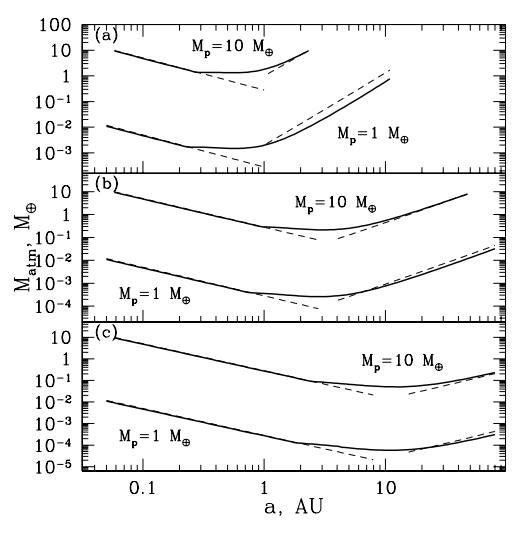
\includegraphics[width=\textwidth]{Mass of Low-Luminosity Atmosphere.png}
\end{column} 
\begin{column}{0.5\textwidth}
This picture shows the difference between out theory(Dashed lines left for equation (58) and right for equation (59)) and simulation(Solid curves).\\
$\alpha=0, \beta=1, \gamma = \frac{7}{5}, \kappa_0=0.1 \text{cm}^2 \text{g}^{-1}$, different panels correspond to different planetesimal accretion regimes: (a) slow, (b) intermediate, and (c) fast.\\
The (a) part of the picture do not fits well, because of the finite size of the core: our extension of the integration in equation (B1) to zero (instead of $R_p$) leads to an overestimate of $M_{atm}$.
\end{column} 
\end{columns}
\end{frame}
\section{Critical Core Mass}
\begin{frame}
\frametitle{Critical Core Mass}
The core will be instable when $M_p \sim M_{atm}$, assuming the exact proportion is $\eta \sim 1$
\begin{equation}
\tag{59}
M_{atm}(M_{cr})=\eta M_{cr}
\end{equation}
In the Low-luminosity case using equations (7), (57), and (A1) we can find:
\begin{equation}
\tag{60}
M_{\text{cr}} \approx \left[ \frac{\eta \theta \Omega \Sigma_p a \kappa_0}{64 \pi^2 \Psi_1 \sigma G^3 M_\odot^{1/3}} \left( \frac{k}{\mu} \right)^{4} \right]^{3/5}
\approx \eta_{0.3}^{3/5} \kappa_{0.1}^{3/5} 
\begin{cases} 
0.26 \, M_\oplus \, a_{10}^{-9/5}&, \text{slow}, \\
25 \, M_\oplus \, a_{10}^{-6/5}&\text{interm.}, \\
240 \, M_\oplus \, a_{10}^{-9/10}&, \text{fast},
\end{cases}
\end{equation}
And in the High-luminosity case using using equation (58), we can find:
\begin{equation}
\tag{61}
M_{cr} = {c_0}^3{(\frac{\eta}{4 \pi \Psi_2 \rho_0 G^3})}^{1/2} \approx 30 M_{\oplus} {\eta_{0.3}}^{1/2} {a_1}^{5/8} 
\end{equation}
\end{frame}

\begin{frame}
\frametitle{Critical Core Mass}
\begin{columns}[t] 
\begin{column}{0.5\textwidth} 
It can also be calculated numerically:
\vspace{-0.1cm}
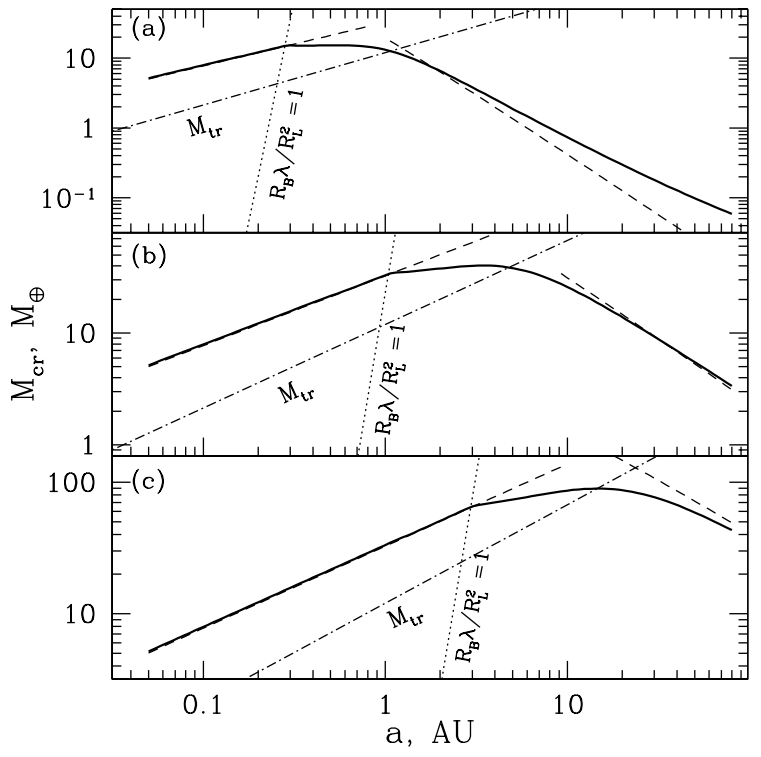
\includegraphics[width=\textwidth]{Critical Core Mass.png}
\end{column} 
\begin{column}{0.5\textwidth}
This picture shows the difference between out theory(Dashed lines left for equation (60) and right for equation (61)) and simulation(Solid curves),besides, the dot-dashed line shows the run of
the transitional mass $M_tr$ with a.\\
different panels correspond to different planetesimal accretion regimes: (a) slow, (b) intermediate, and (c) fast.\\
The (a) part of the picture do not fits well, because of the finite size of the core: our extension of the integration in equation (B1) to zero (instead of $R_p$) leads to an overestimate of $M_{atm}$.
\end{column} 
\end{columns}
\end{frame}
\end{document}
